\documentclass{article}
\usepackage[utf8]{inputenc}
\usepackage{forest}
\usepackage{tikz}
\usepackage{subcaption}
\usepackage{caption}
\usepackage{amsmath}


\title{DARPA Heat Exchanger Model}
\author{Berk Ozturk, Ned Burnell, Bob Haimes}
\date{April 2018}

\begin{document}

\maketitle

\section{Introduction}

We use signomial programming (SP) to design a cross-flow heat exchanger (HX) that takes advantage of the manufacturing capabilities of modern 3D printers. We assume that the heat transfer in each layer in a HX is the same, which means that we can stack layers as required to achieve a certain HX performance. In our diagrams, hot flows runs from south to north, and the cold flow from west to east. 

\section{Models}

\subsection{Levels of abstraction}
\label{ss:abstraction}

We can think of three levels of abstraction in a heat exchanger, which correspond directly to Python GPkit models. 

\begin{itemize}
    \item Cell level (\textbf{HXArea} object)
    \item Channel level (\textbf{RectPipe} object)
    \item Layer level (\textbf{Layer} object)
\end{itemize}

Note that the cell level objects contain multiple fins, which allows us to achieve different levels of fidelity depending on our computational capabilities. 

Then we can organize the models in a hierarchy so that some models inherit the variables and constraints from others, as shown in Figure~\ref{f:hierarchyTree}. These correspond to a total of $(N_{hotpipes}+1) \times (N_{coldpipes}+1)$ GPkit submodels, which are linked together through constraints in the \textbf{Layer} model. 

\begin{figure}
\centering
    \begin{forest}
        [\textbf{Layer}
            [\textbf{ColdPipe}
            [$N_{coldpipes}$]
            ]
            [\textbf{HXArea}
            [$N_{coldpipes} \times N_{hotpipes}$]            
            ]
            [\textbf{HotPipe}
            [$N_{hotpipes}$]
            ]
        ]
    \end{forest}
    \caption{\textnormal{Variable and constraint hierarchy in the SP HX formulation, with number of instances of each model in the leaf nodes.}}
    \label{f:hierarchyTree}
\end{figure}

\begin{center}
\begin{figure}
\centering
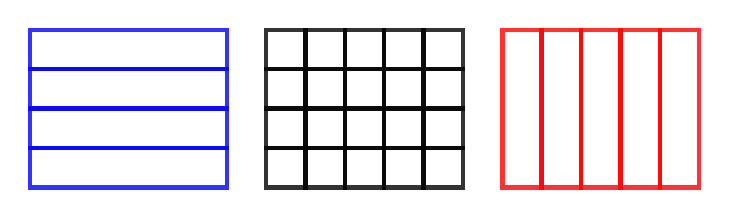
\begin{tikzpicture}[xscale=0.5,yscale=0.5]
\begin{scope}[thick,red]
  \foreach \x in {0,1,2,3,4}
  \draw[ultra thick,red,opacity=.8] (12+\x,0)rectangle(12+\x+1,4);
  
  \foreach \x in {0,1,2,3,4}
  \foreach \y in {0,1,2,3}
  \draw[ultra thick,black,opacity=.8] (6+\x,\y)rectangle(6+\x+1,\y+1);
  
  \foreach \y in {0,1,2,3}
  \draw[ultra thick, blue, opacity=0.8] (0, \y) rectangle (5,\y+1);
\end{scope}
\end{tikzpicture}
\caption{\textnormal{The corresponding geometric abstraction of the vectorized models, demonstrated for 4 cold and 5 hot pipes. Each cell corresponds to an instance of a GPkit model.}}
\end{figure}
\end{center}

\subsection{Partitioning models}

Within the framework described in Section~\ref{ss:abstraction}, we can partition the different types of heat transfer and flow models so that constraints are placed in models that contain and inherit all of the necessary variables. 

\subsubsection{\textbf{Pipe} model}

The \textbf{RectPipe} model defines the channel elements of the heat exchanger, and describes the fluid-wall interactions that result in a transfer of heat. 


%TODO: add full list of constraints in every model? 
%The full set of constraints, in SP-compatible form, are described below:

%\begin{align}
%	\dot{m} &= N_{fins} \times \rho V A \\
%	v_{in} &= v_0 \\
%	V_{out} &= v_{-1} \\
%	v_{avg}^2 &= v_{-} v_{+} \\
%	f_r &= P_f (\frac{1}{2} \rho v_{in}^2) \\
%	P_0_0 &\leq P_{in} + (\frac{1}{2} \rho v_{in}^2) \\
%	P_0_-1 &\leq P_{out} + (\frac{1}{2} \rho v_{out}^2) \\
%	P_0_0 &\leq P_{in} + (\frac{1}{2} \rho v_{in}^2) \\
%\end{align}

\subsubsection{\textbf{HXArea} model}

The \textbf{HXArea} model defines the cells that are defined by the intersection of the pipes. It defines the fluid-wall interface temperature, which differs from the internal temperature of the plate since there is thermal resistance through the plate which has to conduct the heat from one fluid to another. It also makes sure that the individual conductive members of the heat exchanger are not thinner than the minimum thicknesses allowed by a specific method of manufacturing. 

%\begin{align}
%    t_{plate} &\geq t_{min-material} \\
%    t_{hot}  &\geq t_{min-material} \\
%    t_{cold} &\geq t_{min-material} 
%\end{align}

\subsubsection{\textbf{Layer} model}

The \textbf{Layer} model combines the aforementioned \textbf{Pipe} and \textbf{HXArea} models in the HX system. It makes sure that the geometry and heat transfer of the pipes and cells are appropriately linked, and that the outer geometry of the HX is constrained. It also calculates the volume of the material required to manufacture the HX.

\subsection{Inputs to model}

However, different set of inputs can be used to converge the model as long as the unbounded variables described in \textbf{Layer} are appropriately bounded. These are the following:


\subsubsection{Geometric parameters}
\begin{itemize}
\item max solidity: 1-porosity of the HX
\item $x_{dim}$: Maximum x-dimension (cold flow length) of HX
\item $y_{dim}$: Maximum y-dimension (hot flow length) of HX
\item $z_{dim}$
\end{itemize}

\subsubsection{Inlet flow parameters}

\begin{itemize}
\item $v_{in, cold}$: Velocity of incoming cold fluid
\item $v_{in, hot}$: Velocity of incoming hot fluid
\item $P_{in, cold}$: Static pressure of incoming cold fluid
\item $P_{in, hot}$: Static pressure of incoming hot fluid
\item $P_{out, cold}$: Static pressure of outgoing cold fluid
\item $P_{out, hot}$: Static pressure of outgoing hot fluid
\item $D_{hot}$: Drag force on hot side of HX
\item $D_{cold}$: Drag force on cold side of HX
\end{itemize}

\subsubsection{Heat transfer parameters}

\begin{itemize}
	\item $T_{min,cold}$: Minimum temperature of outgoing cold fluid (input if there is a heating requirement)
	\item $T_{max, hot}$: Minimum temperature of outgoing cold fluid (input if there is a cooling requirement)
	\item $T_{in, hot}$: Temperature of incoming hot fluid (can be non-uniform)
	\item $T_{in, cold}$: Temperature of incoming cold fluid (can be non-uniform)
\end{itemize}

\subsection{Objective}

Currently, the objective of the model is the inverse of the total heat transfer. 

\subsection{Use cases for the model}

\begin{itemize}
	\item Design heat exchangers to be built with 3D printing (arbitrary wall thicknesses and cell dimensions).
	\item Do trade studies of different cooling/heating fluids.
    \item Experiment with different materials. 
    \item Determine the sensitivity of heat exchange performance of heat exchanger with respect to inflow/outflow parameters. 
\end{itemize}

\subsection{Future work}

There is plenty to be done to improve the robustness of the optimization method and to generalize it to arbitrary cell tile shapes. 

\end{document}
